% Template for Cogsci submission with R Markdown

% Stuff changed from original Markdown PLOS Template
\documentclass[10pt, letterpaper]{article}

\usepackage{cogsci}
\usepackage{pslatex}
\usepackage{float}
\usepackage{caption}

% amsmath package, useful for mathematical formulas
\usepackage{amsmath}

% amssymb package, useful for mathematical symbols
\usepackage{amssymb}

% hyperref package, useful for hyperlinks
\usepackage{hyperref}

% graphicx package, useful for including eps and pdf graphics
% include graphics with the command \includegraphics
\usepackage{graphicx}

% Sweave(-like)
\usepackage{fancyvrb}
\DefineVerbatimEnvironment{Sinput}{Verbatim}{fontshape=sl}
\DefineVerbatimEnvironment{Soutput}{Verbatim}{}
\DefineVerbatimEnvironment{Scode}{Verbatim}{fontshape=sl}
\newenvironment{Schunk}{}{}
\DefineVerbatimEnvironment{Code}{Verbatim}{}
\DefineVerbatimEnvironment{CodeInput}{Verbatim}{fontshape=sl}
\DefineVerbatimEnvironment{CodeOutput}{Verbatim}{}
\newenvironment{CodeChunk}{}{}

% cite package, to clean up citations in the main text. Do not remove.
\usepackage{apacite}

% KM added 1/4/18 to allow control of blind submission


\usepackage{color}

% Use doublespacing - comment out for single spacing
%\usepackage{setspace}
%\doublespacing


% % Text layout
% \topmargin 0.0cm
% \oddsidemargin 0.5cm
% \evensidemargin 0.5cm
% \textwidth 16cm
% \textheight 21cm

\title{Caregiver reconstruction of children's errors: the preservation of
complexity in language}


\author{Madeline Meyers \and Daniel Yurovsky \\
        \texttt{\{mcmeyers, yurovsky\}@uchicago.edu} \\
       Department of Psychology \\ University of Chicago}

\begin{document}

\maketitle

\begin{abstract}
Why do languages change? One possibility is they evolve due to two
competing pressures: one, for the language to be easily transmitted to
new generations---and hence simple---and another, for the language to be
a useful, descriptive form of communication---and hence more complex.
However, few studies have explored these pressures in the most skilled
language learners: children. Conventional iterated learning studies
focus on the transmission of a novel language from one adult to the
next. However, this ignores one of the important features of language
learning, namely, receiving feedback. This study compares adult
performance on a conventional iterated learning task with their
performance on a task which allows for error correction by a secondary
participant. Results show that adding this error-correcting participant
allows a greater level of complexity to be retained in the language
compared with the baseline task. Data collection is ongoing with
children, but current results suggest that editors (e.g.~parents) may be
playing a dual role in both child language acquisition and language
evolution by re-introducing complexity into a given language.

\textbf{Keywords:}
communication; language acquisition; language evolution; iterated
learning
\end{abstract}

\hypertarget{introduction}{%
\section{Introduction}\label{introduction}}

How do you ask a group of people where they are going in Spanish? In
Spain, the answer depends on the group: you might ask ``Donde van
ustedes?'' of a group of work colleagues, but to address your friends,
you use the informal ``Donde váis vosotros?'' instead. In Mexican
Spanish, this distinction has disappeared, and the ``ustedes'' form is
used exclusively. Why did Spanish change in this way, simplifying and
shedding the formal second person plural? Why do languages change at
all, aside from acquiring new vocabulary? One working theory is that
languages evolve, like biological organisms, to adapt to two dynamic
competing pressures: one, to be easily transmitted and learned (and
hence simple), and another, to be a descriptive and effective system for
communication (and hence complex)(Lupyan \& Dale, 2010).

Children are often the actors who drive language evolution (Senghas,
2003), yet they differ from adults in their 1) cognitive capabilities,
namely, memory systems (Kempe, Gauvrit, \& Forsyth, 2015), 2) interests
and early vocabularies, and 3) conversation partners. Therefore, though
children are skilled language learners, their developing cognitive
systems prevent aspects of language that are difficult to learn and
remember from being passed on---pushing languages towards simplicity
(Hudson Kam \& Newport, 2005; Senghas, 2003). But, languages that become
too simple can lose the ability to be effective for communication
(Kirby, Griffiths, \& Smith, 2014). What enables languages to retain
their communicative utility in the face of these learnability pressures?

The following study tests a novel hypothesis for the maintenance of
structure in language: Communicative inference by caregivers. Children's
language learning is greatly influenced by those around them--especially
the adults they talk to most. These caregivers determine the majority of
their child's language input, and are responsible for seeing that their
children develop effective and useful systems of communication. Even the
youngest children are not passive learners of language---they are active
participants, engaging in conversations with their parents. These adults
are experts both in the language and in the children themselves, as they
understand the child's intuitions, personality, and context. Caregivers
play an important interpretive role in these interactions through their
ability to understand the intended target of children's errorful
productions (Chouinard \& Clark, 2003). They may reconstruct their
child's language in numerous ways-- through explicit or implicit
correction, or simply through modeling correct use of the language over
time (Hudson Kam \& Newport, 2005). By way of this feedback, children's
simplification errors are corrected, and children are able to acquire
adult-like speech. Eventually, when a child grows to be an adult, they
will not transmit the errors they had as a child, but the corrct forms
of speech they learned from their caregivers. Thus, over the course of a
lifetime, the child language learner grows to become a parent language
teacher, correcting their own children's errors. These error
reconstructions may be a mechanism by which more structure is retained
in language over generations than children could sustain alone.

\hypertarget{using-iterated-learning-to-study-language-change}{%
\subsection{Using iterated learning to study language
change}\label{using-iterated-learning-to-study-language-change}}

One way to study language acquisition in the lab is to use the iterated
learning paradigm. This paradigm was created to study the effects of
simplicity and informativity on inter-generational language evolution
(Kirby et al., 2014). In an iterated learning paradigm, one participant
is trained on a randomly-generated language---for example, a set of
words created by arbitrarily pairing syllables together. The participant
is later asked to recall the language, and their responses are given as
training input for the next subject, thus creating a transmission chain.
This iterated process mimics the transmission of language across
generations, with each participant unintentionally changing the language
through their memory biases. Few iterated learning studies, however,
have used children as research subjects. A study by Kempe et al. (2015)
compared child (age 5-8) and adult performances on an iterated learning
task using a novel dot-pattern paradigm. Their results found that
structure emerged faster in children than adults---that is, the
children's patterns simplified much faster than the adult's, allowing
them to be easily reproducable earlier in the transmission chain. This
study provides evidence of the importance of looking at both children
and adults in an iterated learning paradigm, as they have different
cognitive skills which affect their performance in language-learning
tasks (Kempe et al., 2015). However, language evolution cannot be fully
grasped using this paradigm with only separate adult or child learning
chains, because language learning does not occur only within the same
age group (horizontal transmission), or only across age groups (vertical
transmission), but it occurs dynamically, in both directions. In a true
language-acquisition environment, a child receives both language input
and feedback from their caregiver and uses it to interact with their
peers throughout life, eventually growing into a new teacher-caregiver.

The following study uses an iterated learning (diffusion chain) paradigm
with an adaptation of Kempe et al. (2015)'s original non-linguistic task
to investigate how the pressures of descriptiveness and transmissibility
operate in adults when their responses are subject to error correction
by a secondary participant. We hypothesize that these error-correctors
(analogus to caregivers and teachers) are pivotal not only to an
individual's successful language acquisition, but also to the evoulution
of a language as a whole. This is because those who correct mistakes and
provide feedback are able to protect against the transmissibility
(simplicity) bias, which is likely stronger in early language learners,
by re-introuding and preserving complexity in language. All experiments
were pre-registered on Open Science Framework and can be accessed at the
following link: \url{https://osf.io/guzyf/}. {[}Right place to put?{]}

\hypertarget{experiment-1-replicating-kempe-2015}{%
\section{Experiment 1: Replicating Kempe et al.
(2015)}\label{experiment-1-replicating-kempe-2015}}

In a baseline experiment, adults participated in a standard iterated
learning study, using stimuli adapted from Kempe et al. (2015).
Participants were told to reproduce patterns on grids, and each user's
responses were used as training input for the subsequent participant.

\hypertarget{method}{%
\subsection{Method}\label{method}}

\begin{CodeChunk}
\begin{figure}[tb]

{\centering 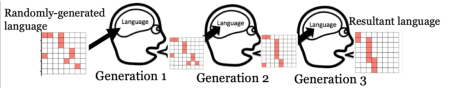
\includegraphics{figs/ill_outline-1} 

}

\caption[In the standard iterated learning paradigm, each participant is trained on input from the previous participant, creating a chain of generational transmission replete with implicit learning errors]{In the standard iterated learning paradigm, each participant is trained on input from the previous participant, creating a chain of generational transmission replete with implicit learning errors. This study uses grid pattern stimuli adapted from Kempe et al. (2015)}\label{fig:ill_outline}
\end{figure}
\end{CodeChunk}

\hypertarget{participants}{%
\subsubsection{Participants}\label{participants}}

Participants in Experiment 1 were 120 adults recruited on Amazon
Mechanical Turk. These participants were dived into twenty diffusion
chains, each of which had six generations. Each participant gave
informed consent, and was compensated with \$0.50 for their
participation.

\hypertarget{design-and-procedure}{%
\subsubsection{Design and Procedure}\label{design-and-procedure}}

Participants in Experiment 1 were told that in this task, they would be
re-creating patterns on a grid. After a consent screen, subjects first
viewed a training trial with two 8x8 grids on the screen -- a target
grid, with 10 cells colored in, and a blank grid. They were told to make
the blank grid match the target grid exactly, and were unable to
progress until the grids were identical. Following this trial,
participants were informed that they would see a target grid appear on
the screen for 10 seconds, followed by a picture (a visual mask)
displayed for 3 seconds. After the visual mask, participants viewed a
blank 8x8 grid where they were given 60 seconds to re-create the target
grid. Participants could click on any cell in the grid to change its
color, and could also undo any color placed. A counter on the screen
showed how many targets had been colored, and it varied dynamicaly with
the participant's clicks. After placing 10 targets, participants could
click a button to adance to the next trial. After completing 3 Practice
trials, which were identical for all partipants in all chains,
participants were informed that the study would begin.

Each participant then completed 6 Experiment trials. Participants in the
first generation of each chain received the same initial grids for
Experiment trials. These initial 8x8 grids were generated by randonly
selecting 10 of the 64 possible cells to be filled. Participants in
subsequent chains received as their targets the outputs produced by
their parent in the chain.

Participants' performance on the practice trials were used as an
attention check to determine whether their data would be passed to the
next participant. If the participant scored less than 75\% accuracy on
the last 2 practice trials, or if they failed failed to select 10 cells
before time ran out, their outputs were not transmitted to the next
generation. {[}HOW MANY Ps were excluded?{]}

\hypertarget{results-and-analysis}{%
\subsection{Results and Analysis}\label{results-and-analysis}}

Our primary measures of interest were reproduction accuracy and pattern
complexity. Reproduction accuracy served as a proxy for transmissibiltiy
-- higher reproduciton accuracies indicate that the ``language'' is
easier to learn. Reproduction accuracy was computed as the proportion of
targets (out of 10) which were placed in the same location on the target
and input grids.

Complexity served as a proxy for descriptiveness. We followed Kempe et
al. (2015) in using several measures of complexity: algorithmic
complexity, chunking, and edge length. Algorithmic complexity is
calculated using the Block Decomposition Method, a measure of
Kolmogorov-Chaitin Complexity applied to 2-dimensional patterns (Zenil,
Soler-Toscano, Dingle, \& Louis, 2014). This measure computes the length
of the shortest Turing machine program required to produce the observed
pattern. The shorter the program, the simpler the pattern. Chunking is
the number of groups of colored blocks which share an edge. The more
groups of blocks, the easier the pattern is to transmit, and the lower
the complexity is. Edge length is the total perimeter of the colored
blocks. If all blocks were in one chunk, the edge length would be low,
and the complexity of the pattern would likely be lower compared to if
none of the chosen targets shared an edge. Implementation of these
metrics was adapted from code used by Gauvrit, Soler-Toscano, \& Guida
(2017).

\hypertarget{results}{%
\subsection{Results}\label{results}}

If iterated learning captures the hypothesized pressures of
expressiveness and transmissibility, we predict that over generations
reproduction accuracy should increase and complexity should decrease. We
tested these predictions with mixed-effects logistic regressions,
predicting accuracy and all three measures of complexity separately from
fixed effects of generation and trial number, and random intercepts for
participant, chain, and initial grid (e.g.
\texttt{accuracy $\sim$ generation + trial + (1|subject) + (1|initial) + (1|chain)}.
{[}NEED SEED AND TRIAL IN MODEL data{]}

Reproduction accuracy increased significantly over generations
(\(\beta =\) 0.025, \(t =\) 3.044, \(p =\) .003). Complexity on all
three measure decreased significantly over generations
(\(\beta_{BDM} =\) -3.22, \(t =\) -6.841, \(p =\) \textless{} .001;
{[}OTHER MEASUERES HERE{]}). Figure \ref{fig:baseline_bothExp_withplots}
shows the results for accuracy and algorithmic complexity.

These findings replicated those found by Kempe et al. (2015).* put in
discussion

\begin{CodeChunk}
\begin{figure}[tb]

{\centering 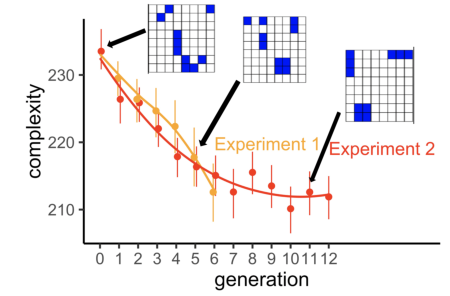
\includegraphics{figs/baseline_bothExp_withplots-1} 

}

\caption[Experiments 1 and 2 show decreases in algorithmic complexity over time]{Experiments 1 and 2 show decreases in algorithmic complexity over time. Experiment 2 begins to asymptote.}\label{fig:baseline_bothExp_withplots}
\end{figure}
\end{CodeChunk}

\hypertarget{experiment-2-baseline-replication}{%
\section{Experiment 2: Baseline
Replication}\label{experiment-2-baseline-replication}}

In Experiment 2, we replicated our task from Experiment 1, but with the
addition of twice as many chains and generations. We replicated the task
with a larger sample in order to determine the shape of the complexity
curve--if it was linear, exponential, or another shape, and if it
reached a stable asymptote of complexity over generations.

\hypertarget{methods}{%
\subsection{Methods}\label{methods}}

Transmission chains consisted of 12 generations each, and there were 40
separate chains. A total of 518 adults participated in this study.
Approximately 7\% (n=38) of participants in the Experiment 2 were
excluded from analysis due to failure to meet accuracy requirements on
the practice trials or failure to select the complete number of targets
on one or more experimental trials. This resulted in a total of 480
participants included in the analysis, four times the number of
participants in Experiment 1.

\hypertarget{results-1}{%
\subsection{Results}\label{results-1}}

The results of this experiment replicated those found in Experiment 1.
Percent accuracy increased linearly over generations (log(generation)
Estimate: 0.05, p \textless{} 0.001), reflecting an increase in
transmissibility of the patterns. Algorithmic complexity, shown in
figure X, appeared to follow an exponential function of the form
{[}format{]} y = e\^{}-x + b. This result was also found in the
alternate measures of complexity (chunking and edge length). The
algorithmic complexity of the patterns decreased, and began to
asymptote. We fit an exponential model (include model formula?), which
was significant (log(generation) Estimate = -0.04, p \textless{} 0.001).

\begin{CodeChunk}
\begin{figure}[tb]

{\centering 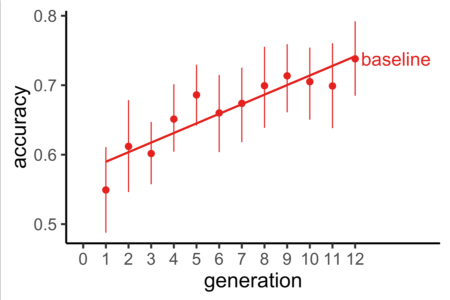
\includegraphics{figs/baseline_accuracy-1} 

}

\caption[Reproduction accuracy increases over generations]{Reproduction accuracy increases over generations.}\label{fig:baseline_accuracy}
\end{figure}
\end{CodeChunk}

\begin{CodeChunk}
\begin{figure}[tb]

{\centering 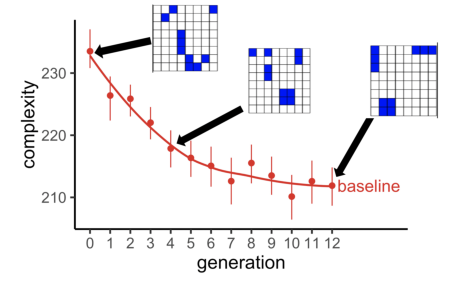
\includegraphics{figs/baseline_withplots-1} 

}

\caption[Algorithmic complexity decreases over time, and reflects simplifications in the patterns produced by participants]{Algorithmic complexity decreases over time, and reflects simplifications in the patterns produced by participants.}\label{fig:baseline_withplots}
\end{figure}
\end{CodeChunk}

\hypertarget{experiment-3-dyad}{%
\section{Experiment 3: Dyad}\label{experiment-3-dyad}}

In order to add an element of error-correction to the iterated-learning
process, we adapted the task from Experiments 1 and 2 to include an
editor participant, analogus to a caregiver who protects their child
from learning incorrect forms of language.

\hypertarget{methods-1}{%
\subsection{Methods}\label{methods-1}}

In the third, dyad experiment, A primary participant was designated as a
``learner'', and completed the same task as in the baseline experiment.
A secondary participant--the ``fixer''--was given an adjusted task,
where instead of reproducing a pattern on a grid, they were told to
``fix the errors'' on a grid pattern in order to match the same target
pattern. The fixer's responses were passed as target input for the
subsequent learner.

Those in the ``fixer'' condition in the dyad experiment were given an
adapted task. The only difference was that throughout the study, they
were not told to re-create the target grid, but to fix a grid they saw
to make it resemble the target grid exactly. Essentially, fixers in the
dyad condition viewed the same target grid as the learners, but instead
of seeing a blank input grid, they saw a grid that already had 10
elements filled in -- the elements that the previous learner had
submitted. The participant could then click and unclick the elements to
edit their positions. There was no ``reset'' button on these patterns,
so they reflect participants first memory instincts.

In the dyad condition, a generation consisted of a learner, who
re-created the target grid, and a fixer, who received the same target
grid as well as the learner's input grid as their grid to edit. The
fixer's final input was used as the target grid for the subsequent
generation.

Transmission chains consisted of 12 generations each, and 40 separate
chains were run during each condition of the study. A total of 1,038
adults participated in this study. Approximately 7\% (n=78) of
participants in Experiment 3 were excluded from analysis due to failure
to meet accuracy requirements on the practice trials or failure to
select the necessary number of targets on one or more experimental
trials. This resulted in a total of 960 participants included in the
analysis.

\hypertarget{results-2}{%
\subsection{Results}\label{results-2}}

We expected to find significant accuracy differences between learners
and fixers: because learners had a more difficult task, the strain on
their working memories was larger, analogous to a child language learner
who is inundated with new words to remember every day. As the fixers had
a less difficult task--they viewed the target as well as what the
learner had produced, we expected their reproduction accuracies to be
greater than the learner's. Additionally, a higher reproduction accuracy
in the learners compared to the fixers would convey that the fixers
were, in fact, correcting errors made by the learners.

Indeed, we see that fixers and learners had significantly different
pattern reproduction accuracies (Fig X). According to a one-way AOV,
these accuracies were sigificantly different (F = 177.3, p \textless{}
0.001). The accuracy of the fixers did not increase significantly over
generations (log(generation) Estimate = -0.01, p = 0.3), while the
accuracy of the learners showed a marginally significant increase
(log(generation) Estimate = 0.02, p = 0.06).

We expected to see a trend in complexity where learners simplified the
language and fixers reintroduced or compensated for some of this loss in
complexity. Indeed, as shown in Figure X, we see this trend.

Overall, we expected to see a smaller decrease in algorithmic complexity
in the fixers over generations compared to in Experiment 2. When fitting
an exponential model to the fixer's complexities, we see a decrease over
generations (log(generation) Estimate = -0.02, p \textless{} 0.001).
Again, the results of algorithmic complexity were in line with those
seen in other measures of complexity (chunking and edge length). This is
significantly different from the results seen in Experiment 2, namely,
the addition of a fixer into the task allowed a higher degree of
complexity to be retained in the language over time (AOV, F = 33.66, p
\textless{} 0.001). Additionally, it appeared that the patterns in the
dyad condition asymptoted sooner than in the baseline condition--the
fixers allowed the language to reach a stable level of complexity
earlier on in the transmission chain.

\begin{CodeChunk}
\begin{figure}[tb]

{\centering 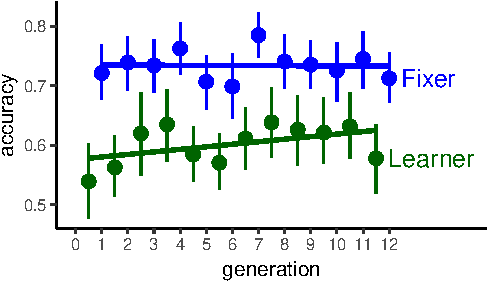
\includegraphics{figs/dyad_accuracy-1} 

}

\caption[In the dyad task, reproduction accuracy stays relatively constant across generations]{In the dyad task, reproduction accuracy stays relatively constant across generations. Fixers have significantly higher accuracies than learners.}\label{fig:dyad_accuracy}
\end{figure}
\end{CodeChunk}

\begin{CodeChunk}
\begin{figure}[tb]

{\centering 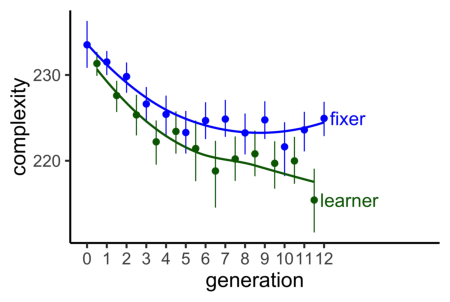
\includegraphics{figs/dyad_complexity-1} 

}

\caption[Fixers reintroudce algorithmic complexity which is lost by learners in the dyad condition]{Fixers reintroudce algorithmic complexity which is lost by learners in the dyad condition.}\label{fig:dyad_complexity}
\end{figure}
\end{CodeChunk}

\begin{CodeChunk}
\begin{figure}[tb]

{\centering 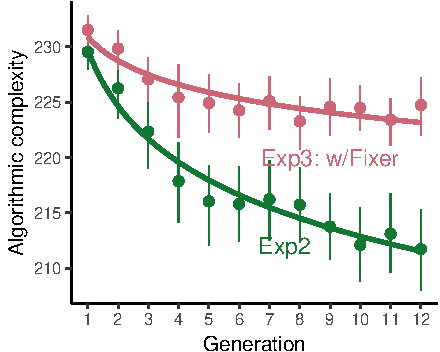
\includegraphics{figs/both_complexity-1} 

}

\caption[The presence of a fixer in the dyad condition causes a much greater level of algorithmic complexity to be retained across the evolution of a novel language]{The presence of a fixer in the dyad condition causes a much greater level of algorithmic complexity to be retained across the evolution of a novel language.}\label{fig:both_complexity}
\end{figure}
\end{CodeChunk}

\hypertarget{general-discussion}{%
\section{General Discussion}\label{general-discussion}}

We do not learn language as passive listeners, who absorb a proportion
of the the linguistic input they hear. Therefore, we cannot measure
language learning only through measuring input, nor through measuring
only linguistic output. Languages are both learned and changed through
conversations, with feedback and error correction, to evolve to the
needs of the language's users. Therefore, we must study language
learning in process, to see how it adapts and evolves with communicative
interactions.

Although Experiments 1-3 used a non-linguistic task, we were able to
measure change in a culturally-transmitted, learned symbol system. In
the baseline experiment, language simplified rapidly and dramatically,
reflecting the strong pressure towards simplification in language
learning. However, when the iterated-learning process begins to resemble
the true process of language-learning, where children speak with and are
subject to correction by those more competent in the language, a lesser
amount of complexity was lost during transmission. In the dyad task, the
fixers represented parents or teachers, as they had an easier memory
task, shown by their higher transmission accuracies. This reflects the
greater ease that adults have when retrieving the correct form of a word
compared to children--their memory for most words is stronger compared
to a child language-learner. The corrected language was passed to the
next learner in the chain, representing a child who, after many years of
being corrected by their own parent, becomes a parent, and, in turn,
passes their optimal language to the next generation. Not only did
editors re-introduce complexity into the language, allowing for a
greater amount of complexity to be retained over time, but they also
helped the language reach an asymptote--a stable level of
complexity--sooner than in Experiments 1 and 2. This stability in
complexity did not mean that the language stopped changing, but that the
descriptiveness and transmissibility pressures were in balance. In fact,
the learner's (analogus to children's) reproduction accuracies were
actually increasing over generations. Despite the stable level of
complexity, learners found the language easier to reproduce over
evolution. Although a high level of descriptiveness was retained in the
language, transmissibility was increasing, without the simplicity
pressure weighing in. Perhaps the language was becoming optimally
complex, with the symbol-patterns changing to be both descriptive and
useful, while being easily transmissible. This reflects the optimal
evolutionary response to these two competing pressures.

When a caregiver or teacher prevents their child from growing up to
believe that ``baba'' is the word for both ``bottle'' and ``sheep'',
they are not only helping their individual child become a competent
speaker of the language, but they are also re-introducing complexity,
and helping the language system as a whole from simplifying to disuse.

\hypertarget{future-directions}{%
\section{Future Directions}\label{future-directions}}

These experiments aim to describe how parents and children uniquely
affect the language evolution process. However, the results described
above were obtained with adult participants. For this reason, we are
currently collecting data with children in both the baseline and dyad
conditions, to see if these pressures operated differently with real
children. Data collection is ongoing with children ages 6-8 at the
Museum of Science and Industry in Hyde Park, Chicago. Children are
participants in the baseline task, and are learners in the dyad task,
with adult mTurkers as the fixers. Children complete the task on an
iPad, and receive their choice of stickers as compensation. iPad tasks
have many advantages over other research methods, including the
paper-and-sticker task used by Kempe et al. (2015) because the use of an
iPad reduces the completion time of the study and is engaging for young
children (Frank, Sugarman, Horowitz, Lewis, \& Yurovsky, 2016). Parents
of the children in the study completed an additional child information
sheet about the child's language experiences and home environment. We
expect to see similar trends in complexity over time with children as
were seen with adults, namely, that in the dyad task, adults reintroduce
complexity which is lost by child language learners. However, we expect
sharper initial decreases in complexity with children, in line with the
findings of Kempe et al. (2015). We plan to conduct a set of qualitative
analyses on the patterns produced by adults and children, in order to
see whether children are simply making more errors than adults, or if
they are making fundamentally different errors, perhaps reflecting their
differential cognitive language-learning systems.

\vspace{1em} \fbox{\parbox[b][][c]{7.3cm}{\centering All code for these analyses are available at\ \url{https://github.com/mcmeyers/iteratedlearning}}}

\hypertarget{acknowledgements}{%
\section{Acknowledgements}\label{acknowledgements}}

This research was funded by a James S. McDonnell Foundation Scholar
Award to DY.

\hypertarget{references}{%
\section{References}\label{references}}

\setlength{\parindent}{-0.1in} 
\setlength{\leftskip}{0.125in}

\noindent

\hypertarget{refs}{}
\leavevmode\hypertarget{ref-chouinard-2003}{}%
Chouinard, M. M., \& Clark, E. V. (2003). Adult reformulations of child
errors as negative evidence. \emph{Journal of Child Language},
\emph{30}(3), 637--669.

\leavevmode\hypertarget{ref-frank-2016}{}%
Frank, M. C., Sugarman, E., Horowitz, A. C., Lewis, M. L., \& Yurovsky,
D. (2016). Using tablets to collect data from young children.
\emph{Journal of Cognition and Development}, \emph{17}(1), 1--17.

\leavevmode\hypertarget{ref-gauvrit-2017}{}%
Gauvrit, N., Soler-Toscano, F., \& Guida, A. (2017). A preference for
some types of complexity comment on ``perceived beauty of random texture
patterns: A preference for complexity''. \emph{Acta Psychologica},
\emph{174}, 48--53.

\leavevmode\hypertarget{ref-hudsonkam-2005}{}%
Hudson Kam, C. L., \& Newport, E. L. (2005). Regularizing unpredictable
variation: The roles of adult and child learners in languagae formation
and change. \emph{Language Learning and Development}, \emph{1}(2),
151--195.

\leavevmode\hypertarget{ref-kempe-2015}{}%
Kempe, V., Gauvrit, N., \& Forsyth, D. (2015). Structure emerges faster
during cultural transmission in children than in adults.
\emph{Cognition}, \emph{136}, 247--254.

\leavevmode\hypertarget{ref-kirby-2014}{}%
Kirby, S., Griffiths, T., \& Smith, K. (2014). Iterated learning and the
evolution of language. \emph{Current Opinion in Neurobiology},
\emph{28}, 108--114.

\leavevmode\hypertarget{ref-lupyan-2010}{}%
Lupyan, G., \& Dale, R. (2010). Language structure is partly determined
by social structure. \emph{PLoS ONE}, \emph{5}(1), 1--10.

\leavevmode\hypertarget{ref-senghas-2003}{}%
Senghas, A. (2003). Intergenerational influence and ontogenetic
development in the emergence of spatial grammar in nicaraguan sign
language. \emph{Cognitive Development}, \emph{18}, 511--531.

\leavevmode\hypertarget{ref-zenil-2014}{}%
Zenil, H., Soler-Toscano, F., Dingle, K., \& Louis, A. A. (2014).
Correlation of automorphism group size and topolical properties with
program-size complexity evaluations of graphs and complex networks.
\emph{Physica A}, \emph{404}, 341--358.

\bibliographystyle{apacite}


\end{document}
